
\chapter{Validation}
\section{Validation Strategy}
Model validation could be considered an important step towards creating a robust and useful simulation tool, though there is little dedicated literature referring to the process of successfully validating wave solving acoustic simulation software. A greater volume of literature is availalbe for the validation of Ray based methods such as~\cite{Ahnert2005,Tsingos2002,Foteinou2010}, and the validation of a hybrid scheme by Murphy \textit{et al} is available ~\cite{Southern2013}. Studies such as Hill~\cite{Hill2012}. This section will review an attempt to validate the FDTD and PSTD tools described above, with a small 3D domain.\\

\subsection{The Domain}
The domain used for validation in this study was a fully bounded room with the following properties:\\

\begin{itemize}
\item Length $L_x = 5m$
\item Width $L_x = 4m$
\item Height $L_z = 3m$
\item Volume = $ v = 60m^3$
\item Surface Area $S_{area} = 94m^2$
\item Uniform Absorption Coefficient $\alpha = 0.45 $
\item Schroeder Frequency  $f_{schroeder} = 107Hz $,
\item The Reflection Order $N_{reflections} = 30.7$
\item Mean Free Path Between Reflections $MFP = 2.55m$
\item Eyring Reverberation Time $RT_{60} = 0.1719s $
\end{itemize}

The axial, tangential and oblique modes below the Schroeder frequency are calculated as:\\
\begin{figure}[H]
\centering
  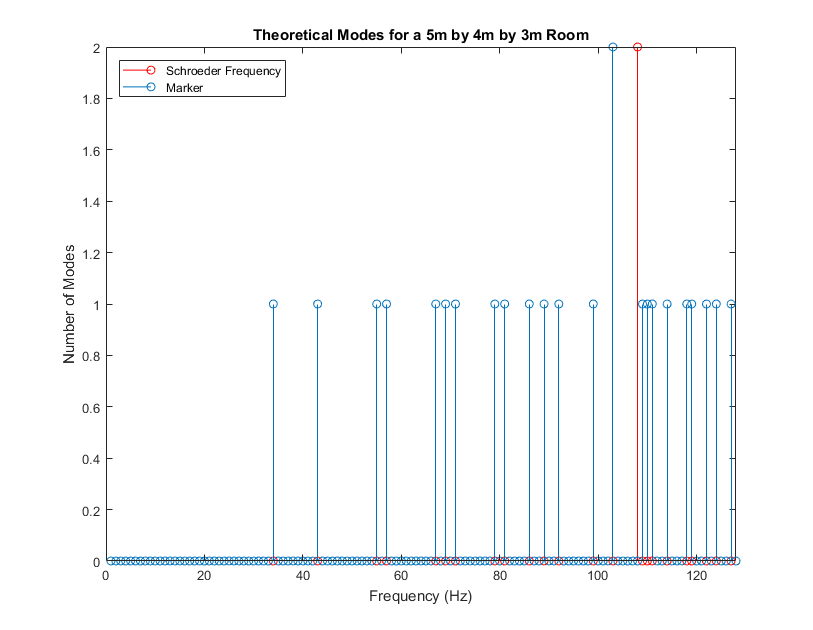
\includegraphics[width=\textwidth]{./graphics/modesuptoschr.png}
  \caption{Room Modes up to Schroeder Frequency for a Small Rectangular Room}
\end{figure}

The stimulus position in each domain was $1.0m$ in each direction from the bottom left corner, and the receiver position was the exact middle of the domain. The stimulus source type was a soft source, as described in the time domain numerical methods section above. 
The source content was an MLS sequence of 11th order with 2 repetitions. The MLS signal was generated using the MLS toolbox by MRP Thomas~\cite{Mrt2008}. The signal was normalised with a Gaussian window to the length of the signal array. The maximum frequency of interest in this validation was $5kHz$, giving a $0.333e^{-5}$ step time for the FDTD simulation, and a $0.1e^{-4}$ step time for the PSTD simulation.

\subsection{Post Processing}
The aim of the validation was be to show that there is minimal error in the normalised power spectral density between source and receiver location. This will show that waves are travelling from source to receiver without aliasing or unexpected loss in the frequency range of interest. Some modal influence was expected, as is DC offset. To reduce the effect of the DC term, a DC blocking filter was used when post processing the source and receiver recorded signals. This filter was generated using the Matlab filter design tool. As with ~\cite{Murphy2014} the input and output signals on the grid were recorded, and the signals are normalised to each other.\\

\section{Results}
Below is a plot of the spectral power of the source signal, the FDTD receiver position and the PSTD receiver position for the simulation described above. The normalised input and output subplot in these figures is shifted in time to remove the time lag between source and receiver locations.

\begin{figure}[H]
\centering
\textbf{FDTD Validation Data}
  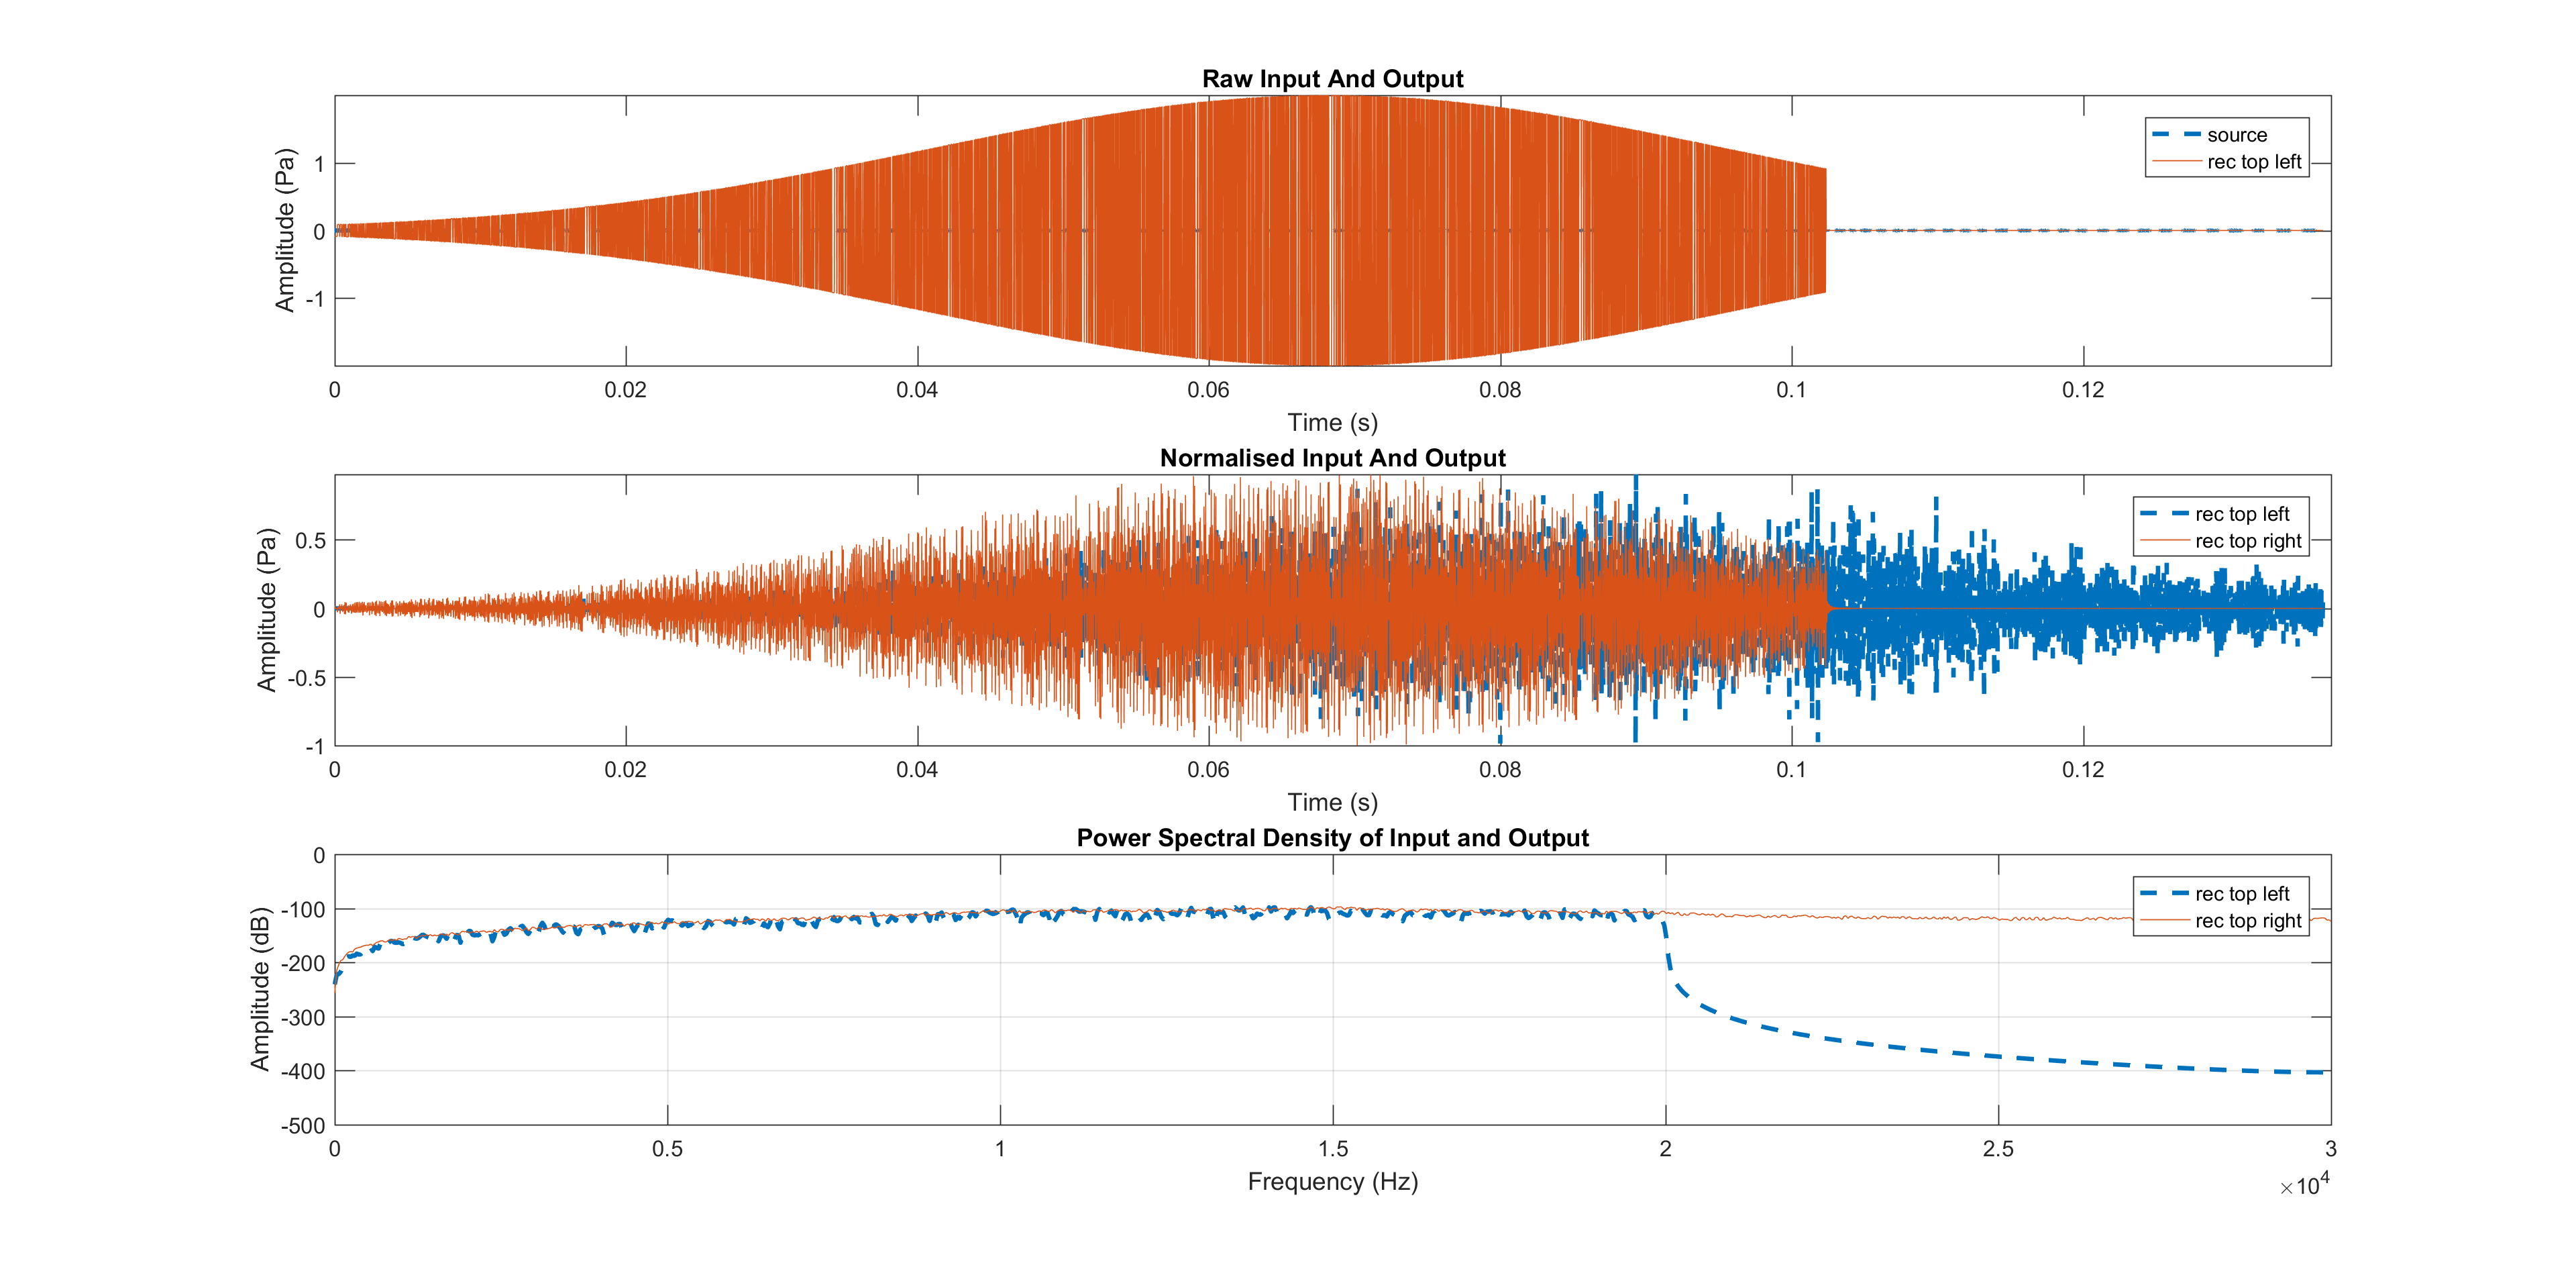
\includegraphics[width=\textwidth]{./graphics/FDTDvalidationFinal.png}
  \caption{Validation data of FDTD simulation}
\end{figure}

\begin{figure}[H]
\centering
\textbf{PSTD Validation Data}
  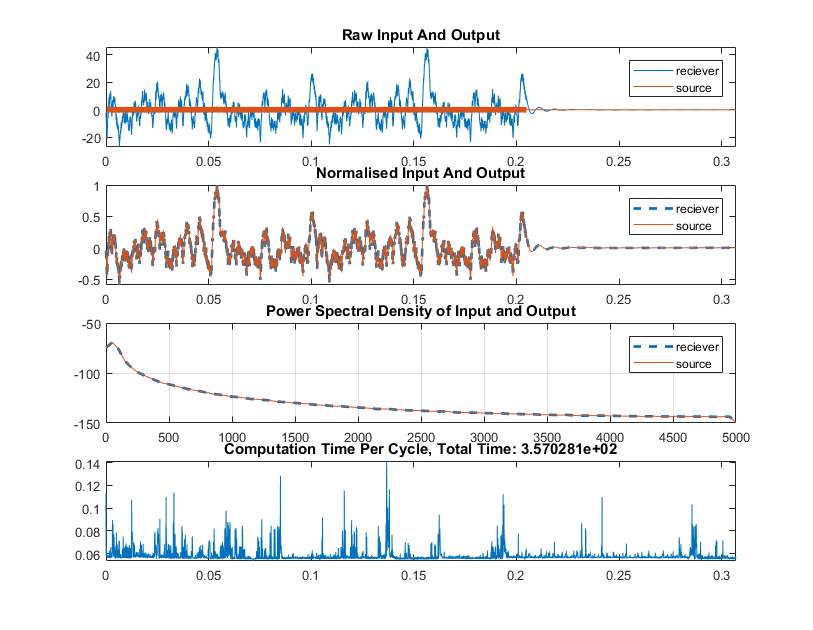
\includegraphics[width=\textwidth]{./graphics/PSTDvalidation10k.png}
  \caption{Validation data of PSTD simulation}
\end{figure}

It can be seen that both simulations have reasonably good agreement between the power spectral densities (PSD) of the source and receivers in the frequency region of interest. There is a significant low frequency signal present in the PSTD response, in both the source and receiver sections.  Due to the 6 steps per wavelength of the FDTD simulation, the time step was also smaller than for the PSTD simulation. As such when using Matlabs Pwelch function to perform PSD estimation, the estimation was made beyond the frequency range of interest.\\


\section{Validating The SFDTD Method}
As the SFDTD method was implemented only to 2D and it could not be validated with the 3D FDTD and PSTD methods as above. The SFDTD method was tested using a 5m by 4m domain, with absorption coefficients of $ \alpha = 0.45$. The signal used was a chirp that was generated using the Chip function of the Matlab DSP Systems Toolbox, with a start frequency of 100Hz and a stop frequency of half the maximum target frequency (or a quarter of Nyquist), that was normalised to $100dBSPL$ and has a sweep time of $0.4s$. Before normalisation, a Hamming window was applied to the signal to minimize the discontinuity of introducing the source. The figure below presents the output data for the SFDTD validating simulation:\\

\begin{figure}[H]
\centering
\textbf{PSTD Validation Data}
  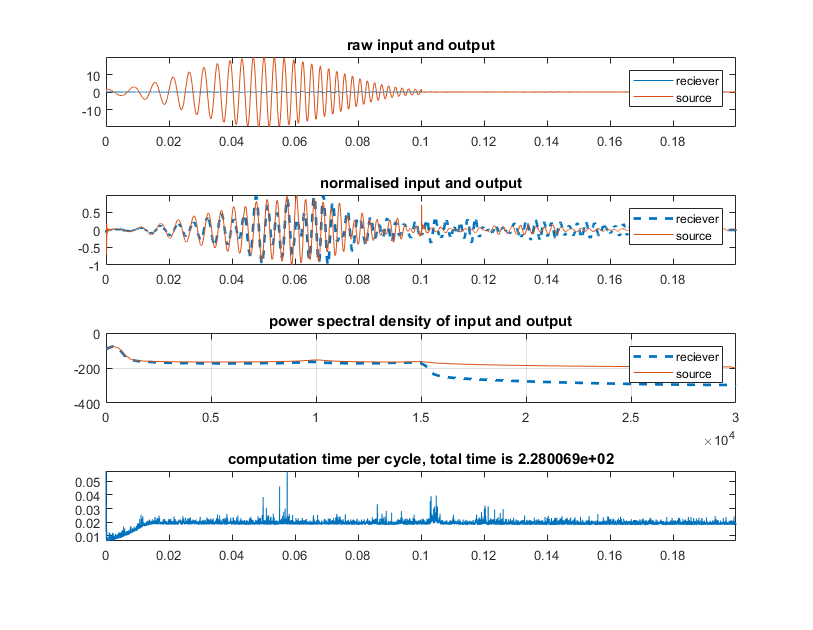
\includegraphics[width=\textwidth]{./graphics/SFDTDvalidationFinal.png}
  \caption{Validation data of PSTD simulation}
\end{figure}
As with the PSTD method there is a shared low frequency component, but the PSD between source and receiver are very close to well beyond the highest frequency of interest.